\documentclass{../pdae} %\documentclass[12pt]{../pdae}
% Necesario aquí para que lea bien el shorttitle
% Título en la cabecera

\shorttitle{Pràctica 3:\\Timers i Interrupcions}
\title{Creació de Funcions de Retard i un Rellotge en Temps Real mitjançant
l’ús de Timers i Interrupcions}

\author{
    Iván Canales\\
    Xavier Ripoll
}

\date{23 de març de 2018}

\begin{document}
\maketitle

\section{Introducció}

\subsection{Objectius}
% Què es vol fer a la pràctica.

La pràctica té dues parts principals.

Abans de fer cap de les dues, ens cal configurar els \textit{timers} del
microcontrolador per tal de poder utilitzar-los.

En el primer exercici, refactoritzem la part del
codi de la pràctica 2 en què es permetia modificar la freqüència i direcció
dels LEDs de la placa inferior. La idea és emprar els \textit{timers} del
microcontrolador per mesurar el temps amb més precisió i controlar millor
els casos excepcionals (e.g. quan al pujar o baixar la freqüència hi ha un
\textit{overflow} o \textit{underflow}).

La segona part consisteix en dissenyar tant la interfície (per la pantalla LCD)
com la implementació (novament amb \textit{clocks} i \textit{timers}) d'un
rellotge que porti l'hora i una alarma, ambdues programables.

Com a petita indicació, expliquem aquí com funcionen els \textit{inputs} per
poder emprar correctament el sistema de rellotge i alarma:

En pantalla es mostraran dos nombres amb el format:

\begin{lstlisting}
 hora HH:MM:SS
            ##
 alarma HH:MM

\end{lstlisting}

On \texttt{HH:MM:SS} mostra l'hora del rellotge i \texttt{HH:MM} l'alarma
programada amb precisió de minut, com es demana a l'enunciat de la pràctica.

Els dos coixinets (\texttt{\#\#}) subratllen el camp que volem modificar.
Amb el \textit{joystick} esquerra i dret canviem als camps dels costats,
mentre que amb adalt i abaix incrementem i decrementem (corresponentment)
el valor. Prement el botó S1 seleccionem el rellotge, mentre que amb S2
seleccionem l'alarma.

Per evitar conflictes de sincronisme, cal pausar el rellotge abans
de poder modificar-lo. Prèmer el \textit{joystick} alterna l'estat de pausa
del rellotge.

\subsection{Recursos utilitzats}
% Quins recursos del Microcontrolador, Placa d’Experimentació i Robot es fan servir.
Utilitzarem el \texttt{SMCLK} com a \textit{clock} base per al \textit{timer}
que controla els LEDs i el rellotge \texttt{ACLK} per controlar l'hora i
l'alarma. Aquesta decisió és deguda a que necessitem una freqüència molt més alta
pel rellotge dels LEDs (1000Hz) que pel que porta l'hora (1Hz).

De la placa \textit{Boosterpack MK II} volem fer servir tant el
\textit{joystick} com els polsadors S1 i S2 com a entrades, a més a més de la
pantalla LCD com a sortida (en la que es mostrarà la freqüència dels LEDs,
l'hora i l'alarma).

De la placa d'experimentació, novament farem servir els vuit LEDs del port P7
per mostrar la llum que es va ``desplaçant''.


\subsection{Configuració dels recursos}
% Com s’han configurat els diferents recursos.
\subsubsection{Configuració dels LEDs, botons i \textit{joysticks}}

La fem de forma idèntica a la pràctica anterior, degut a que la programació
de l'efecte que tenen els \textit{inputs} està al \texttt{main} i no
a les rutines d'interrupció.

\subsubsection{Configuració dels \textit{timers}}
Abans de configurar els timers, cridem la funció \texttt{init\_ucs\_24MHz} per
a que inicialitzi el \textit{unified clock system}.

En els dos \textit{timers} s'ha usat mode \textit{pull up}. Com ja hem comentat,
per al \textit{timer} dels LEDs usem el \textit{clock} de freqüència alta i
pel de l'hora el \textit{clock} de freqüència baixa.

En ambdós casos hem usat un divisor de freqüència de valor 8 perquè el valor
dels \texttt{CCR}s no sigui massa alt, seguint el raonament següent:

\begin{equation*}
  CCR = \frac{F}{fd}
\end{equation*}

On $CCR$ és la constant \texttt{CCR} que marca quants cicles fa el comptador
abans de tornar a 0; $F$ és la freqüència del rellotge; $f$ la freqüència que
volem aconseguir; i $d$ el divisor de freqüència.

En el cas del \textit{timer} dels LEDs, tenim:

\begin{equation*}
  CCR = \frac{24\times10^{6}\mathrm{Hz}}{1000\mathrm{Hz}\times 8} = 3000
\end{equation*}

En l'altre \textit{timer}, trobem:

\begin{equation*}
  CCR = \frac{2^{15}\mathrm{Hz}}{1\mathrm{Hz}\times 8} = 4096
\end{equation*}


\subsection{Funcions utilitzades}
% Com i per quines funcions es fan servir.

Per aquesta pràctica hem decidit modularitzar lleugerament el codi, separant
el "cos" del \texttt{main} a una funció \texttt{manage\_states} que s'encarrega
de canviar l'\textit{output} en funció de l'estat actual.

La resta de funcions són heretades de la pràctica anterior, entre elles
destaquen els \textit{handlers} de les interrupcions i les funcions de
configuració del \textit{hardware}.

\subsection{Problemes}
% Problemes que han sorgit (que no siguin de compilació) i com s’han solucionat.
El problema principal amb el que ens vam trobar, va ser el fet que si es vol
modificar el temps del rellotge, era possible que es produís un canvi en el
camp que es vol modificar (passa un segon, per exemple) i llavors el canvi de
temps no tenia el funcionament esperat. Per a solucionar-ho, vam introduir la
funció d'aturar el rellotge, i per a modificar el temps serà necessari
pausar-lo primer.

\subsection{Conclusions}

La configuració i ús dels \textit{timers} i interrupcions ens ha semblat
sorprenentment senzilla en comparació a l'experiència que vam tenir realitzant
la pràctica anterior. Això ens fa creure que gran part de la dificultat que
patim en programar el microcontrolador es deguda més aviat a la corba
d'aprenentatge que a la complicació que presenta en sí.

També hem intentat netejar i ordenar el codi per poder reutilitzar-lo el
màxim possible en les properes pràctiques.

\section{Comentari del codi}

\subsection{Inicialització i ús dels timers}

En aquesta pràctica farem servir dos \textit{timers} diferents, el
\texttt{TA0} i el \texttt{TA1}. En conseqüència, cal que els activem en els
tres nivells.

En el primer nivell, farem servir una funció \texttt{init\_timer} que
configurarà els \textit{timers} per a que facin servir el clock (\texttt{SMLK}
pel \textit{timer} 0 i \texttt{ACLK} pel \textit{timer} 1), el mode \texttt{UP}
i un divisor adient (8 en aquest cas). A més, com volem comptar fins a 1 segon
o 1 mil·lisegon (pels \textit{clocks} 1 i 0 respectivament), cal que posem un
valor adequat a \texttt{TAxCCR0}.

\begin{lstlisting}[language=C]
void init_timer(void) {

    /****** Timer 0 ******/
    // Retraso de los LEDs

    TA0CTL =
            TASSEL__SMCLK + // clock SMCLK
            MC__UP +        // modo UP
            ID__8;          // /8

    TA0CCTL0 =
            CCIE; // activar int clock

    // Ponemos la constante de tiempo maximo del contador
    // Lo ponemos a 3000 ya que f/1000/8 = 24*10^6/1000/8 = 3000
    TA0CCR0 = 3000;

    /****** Timer 1 ******/
    // hh:mm:ss y alarma

    TA1CTL =
            TASSEL__ACLK + // clock SMCLK
            MC__UP +       // modo UP
            ID__8;         // /8

    TA1CCTL0 =
            CCIE; // activar int clock

    // Seteamos la constante de tiempo maximo del contador
    // Lo ponemos a 4096 ya que f/8 = 2^15/8 = 4096
    TA1CCR0 = 4096;
}
\end{lstlisting}

A continuació, per configurar la resta de nivells de la interrupció, ampliarem
la funció \texttt{init\_interrupciones} per a que consideri els dos
\textit{timers} que volem configurar.
Notem que \texttt{BIT8} farà referència al \textit{timer} dels leds, i
\texttt{BITA} al timer del rellotge. Finalment, es fa una crida a
\texttt{\_\_enable\_interrupt}.

\begin{lstlisting}[language=C]
void init_interrupciones()
{
 	/* [...] */

    // Timer leds
    NVIC->ICPR[0] |= BIT8; //Primero, me aseguro de que no quede ninguna interrupcion residual pendiente para este puerto,
    NVIC->ISER[0] |= BIT8; //y habilito las interrupciones del puerto

    // Timer hora
    NVIC->ICPR[0] |= BITA; //Primero, me aseguro de que no quede ninguna interrupcion residual pendiente para este puerto,
    NVIC->ISER[0] |= BITA; //y habilito las interrupciones del puerto

    __enable_interrupt(); //Habilitamos las interrupciones a nivel global del micro.
}
\end{lstlisting}

Per les interrupcions que provoquen cadascun dels \textit{timers} al passar
el temps indicat, creem dos \textit{handlers} (\texttt{TA0\_0\_IRQHandler} i
\texttt{TA1\_0\_IRQHandler}). El primer serà cridat cada mil·lisegon mentre que
l'altre cada segon, d'acord amb la configuració abans especificada. Aquest
últim, a més de fer increments de 1 cada cop que es cridat, també tornarà a
0 quan arribi a 86400 (és a dir, un dia sencer), per a que el rellotge torni
a marcar les 00:00.

\begin{lstlisting}[language=C]
/**
 * Handler del timer que se activa cada ms.
 * Este timer se usara para el delay de los leds
 **/
void TA0_0_IRQHandler(void) {
    TA0CCTL0 &= ~CCIE; // Desactivamos interrupciones

    ms_elapsed++; // Ha pasado 1ms

    TA0CCTL0 &= ~CCIFG; // Limpiar flag
    TA0CCTL0 |=  CCIE;  // Reactivamos interrupciones
}

/**
 * Handler del timer que se activa cada segundo.
 * Este timer se usara para el reloj y la hora
 **/
void TA1_0_IRQHandler(void) {
    TA1CCTL0 &= ~CCIE; // Desactivamos interrupciones

    time_seconds++; // Ha pasado 1s
    time_seconds %= 86400; // Un dia = 86400s

    TA1CCTL0 &= ~CCIFG; // Limpiar flag
    TA1CCTL0 |=  CCIE;  // Reactivamos interrupciones
}
\end{lstlisting}
\textit{Cal notar que \texttt{ms\_elapsed} és una variable global que compta
els mil·lisegons que han passat.}

% TODO (no a aqui necessariament) explicar com funcionen els inputs! i fer diagrama dels outputs per pantalla?

\section{Diagrames de flux}

S'inclouen els diagrames del \texttt{main} i les subrutines que inclou.

Els nous \textit{handlers} afegits solament incrementen constants com ja s'ha
esmentat a la secció de comentari del codi.

\begin{figure}[H]
  \centering
  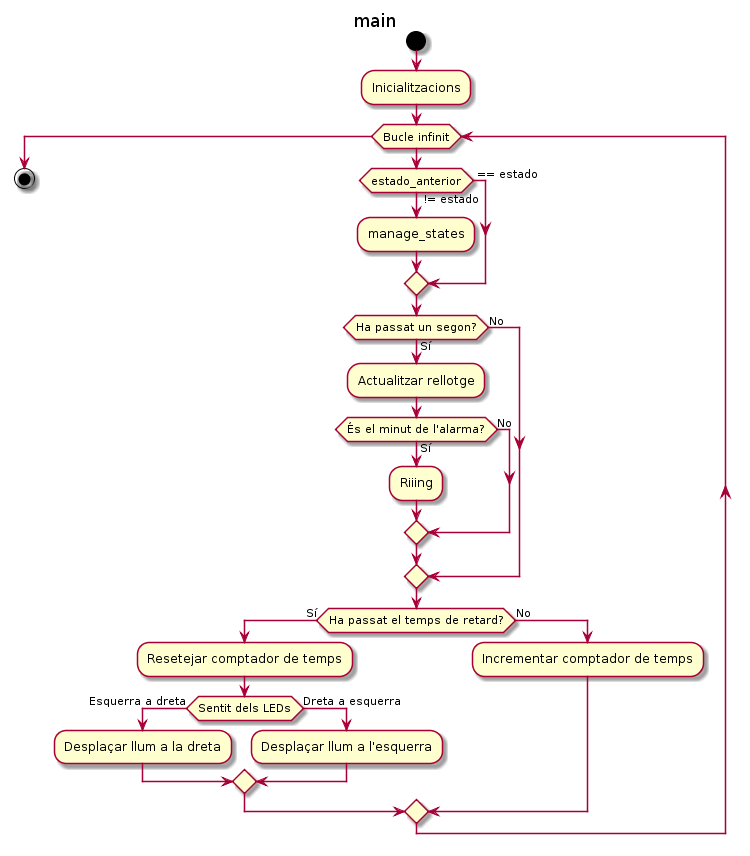
\includegraphics[scale=.45]{main}
\end{figure}

\begin{figure}[H]
  \centering
  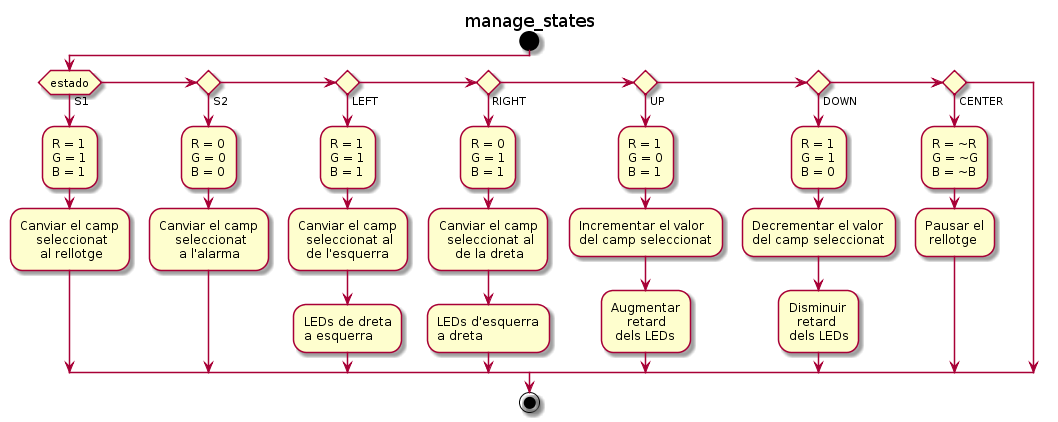
\includegraphics[scale=.4]{manage_states}
\end{figure}

\end{document}
